\documentclass[11pt,a4paper]{article}

% ==================== PAQUETES ====================
\usepackage[utf8]{inputenc}
\usepackage[T1]{fontenc}
\usepackage[spanish]{babel}
\usepackage{geometry}
\geometry{left=3cm, right=3cm, top=2.5cm, bottom=2.5cm}
\usepackage{setspace}
\usepackage{graphicx}
\usepackage{titlesec}
\usepackage{parskip}
\usepackage{helvet}
\renewcommand{\familydefault}{\sfdefault}
\usepackage{hyperref}
\usepackage{xurl}      % rompe URLs largas
\hypersetup{
    colorlinks=true,
    linkcolor=blue,
    urlcolor=blue,
    citecolor=blue
}
\usepackage{graphicx}
\usepackage{float}
\usepackage{microtype}
\usepackage{tikz}
\usepackage{xcolor}
\usepackage{tcolorbox}
\tcbuselibrary{skins}
\usepackage{fancyhdr}
\usepackage{enumitem}
\usepackage{amsmath}
\usepackage{booktabs}
\setlength{\abovedisplayskip}{5pt}
\setlength{\belowdisplayskip}{6pt}
\setlength{\abovedisplayshortskip}{4pt}
\setlength{\belowdisplayshortskip}{4pt}

% ==================== COLORES ====================
\definecolor{azuloscuro}{RGB}{10, 50, 100}
\definecolor{azulmedio}{RGB}{25, 65, 120}
\definecolor{dorado}{RGB}{180, 145, 60}
\definecolor{grisclaro}{RGB}{245, 245, 245}

% ==================== CONFIGURACIÓN ====================
\setstretch{1}
\pagestyle{fancy}
\fancyhf{}
\fancyfoot[C]{\thepage}   % Número centrado en el pie
\renewcommand{\headrulewidth}{0pt}

\titleformat{\section}
    {\normalfont\Large\bfseries\color{azuloscuro}}{\thesection.}{0.5em}{}
\titleformat{\subsection}
    {\normalfont\large\bfseries\color{azulmedio}}{\thesubsection.}{0.5em}{}

\titlespacing*{\section}
{0pt}{2.0ex plus 0.5ex minus 0.2ex}{1.0ex}

\titlespacing*{\subsection}
{0pt}{1.2ex plus 0.3ex minus 0.2ex}{0.5ex}

\begin{document}

% ==================== PORTADA ====================
\begin{titlepage}
% --- FONDO Y ELEMENTOS DECORATIVOS ---
\begin{tikzpicture}[remember picture, overlay]
    
    % 1. Barra lateral decorativa (se dibuja primero para quedar al fondo)
    \fill[azulmedio] (current page.north west) rectangle ([xshift=1.2cm]current page.south west);
    
    % 3. Línea dorada decorativa superior
    \fill[dorado] ([yshift=-6cm]current page.north west) rectangle ([yshift=-6.15cm]current page.north east);
    
    % 4. Caja inferior gris
    \fill[grisclaro] (current page.south west) rectangle ([yshift=3.9cm]current page.south east);
    
    % 5. Línea dorada decorativa inferior (para equilibrar el diseño)
    \fill[dorado] ([yshift=3.9cm]current page.south west) rectangle ([yshift=3.8cm]current page.south east);

        % 2. Fondo azul oscuro en la parte superior
    \fill[azuloscuro] (current page.north west) rectangle ([yshift=-6cm]current page.north east);
    \node[anchor=center] at ([xshift= 2.4 cm, yshift=-2.9 cm]current page.north west) {
\includegraphics[width=3.7cm]{complejo.png}};
    
    % --- TEXTOS ENCABEZADO Y PIE (Posicionamiento Absoluto) ---
    % Se ajusta xshift=0.6cm para centrar visualmente restando la barra lateral
    
    % Texto Superior (Institución)
    \node[anchor=center, text=white, align=center] at ([yshift=-3cm, xshift=1 cm]current page.north) {
        % \includegraphics[width=3cm]{logo.png} \\[0.3cm] % Descomenta si usas logo
        {\scshape\LARGE Complejo Educativo Thomas Jefferson}\\[0.3cm]
        {\scshape\large Infraestructura Tecnológica y Servicios Informáticos}
    };

    % Texto Inferior (Lugar y Fecha)
    \node[anchor=center, text=azuloscuro, align=center] at ([yshift=1.75cm, xshift=0.6cm]current page.south) {
        {\large\scshape Sonsonate, El Salvador}\\[0.15cm]
        {\large Junio 2026}\\[0.35cm]
    };
    
\end{tikzpicture}

% --- CONTENIDO CENTRAL DE LA PÁGINA ---

% Espacio para saltar el banner superior (6.15cm)
\vspace*{5cm}

\begin{center}
    \begin{tcolorbox}[
        enhanced,
        colback=white,
        colframe=azuloscuro,
        width=0.9\textwidth,
        arc=4mm,
        boxrule=1.5pt,
        drop shadow=azuloscuro!30!white, % Sombra suavizada e integrada
        borderline={0.5pt}{3pt}{dorado}, % ¡NUEVO! Detalle de borde interno dorado
        left=20pt,
        right=20pt,
        top=20pt,
        bottom=20pt
    ]
        \centering
        % ¡NUEVO! Líneas separadoras en dorado para mayor elegancia
        {\color{dorado}\rule{0.6\textwidth}{1pt}}\\[0.6cm]
        {\Huge\bfseries\color{azuloscuro} El impacto de la seguridad
        en el crecimiento económico\\[0.6cm]
        de El Salvador}\\[0.6cm]
        {\color{dorado}\rule{0.6\textwidth}{1pt}}\\[0.4cm]
        {\Large\itshape\color{azulmedio} Documento de investigación}
    \end{tcolorbox}
\end{center}



% --- INFORMACIÓN DE AUTORÍA ---
\begin{center}
    \vspace{2cm}
    {\large\bfseries\color{azuloscuro} Presentado por:}\\[0.15cm]
    {\Large Mario Alejandro Marroquín Meléndez}\\[0.8cm]

    {\large\bfseries\color{azuloscuro} Línea de investigación:}\\[0.15cm]
    {\large Economía del Desarrollo}
\end{center}

% Espacio inferior para evitar que el texto toque el banner gris
\vspace*{2.5cm}

\end{titlepage}
% 

\section*{Introducción}
\addcontentsline{toc}{section}{Introducción}

La relación entre seguridad, calidad institucional y desarrollo económico ha ocupado un lugar central dentro de la economía del desarrollo durante las últimas décadas. La literatura sobre economía institucional sostiene que el crecimiento económico depende, en gran medida, de la capacidad de las instituciones para garantizar el Estado de Derecho, proteger los derechos de propiedad y generar un entorno predecible para la inversión y la actividad productiva (North, 1990; Rodrik et al., 2004; Acemoglu \& Robinson, 2012). En este contexto, sociedades más seguras tienden a ofrecer mejores condiciones para la inversión, fortalecer el funcionamiento institucional y favorecer un crecimiento económico sostenido (World Bank, 2011).

Sin embargo, investigaciones más recientes plantean que la seguridad no constituye únicamente un determinante directo del desempeño económico, sino también una manifestación observable de la capacidad institucional de un Estado para hacer cumplir la ley, controlar la corrupción y mantener la estabilidad política (Kaufmann et al., 2010; World Bank, 2011). Desde esta perspectiva, la violencia no representa únicamente un problema de seguridad pública, sino un síntoma del funcionamiento de las instituciones encargadas de garantizar el orden jurídico y la gobernabilidad.

En consecuencia, la violencia puede entenderse como un indicador de debilidad institucional. Países con elevados niveles de criminalidad suelen presentar mayores dificultades para hacer cumplir la ley, menores niveles de confianza en las instituciones y un entorno menos favorable para la inversión y el desarrollo productivo (World Bank, 2011; UNODC, 2023). Asimismo, la evidencia internacional muestra que la calidad institucional constituye uno de los principales determinantes de las diferencias de desarrollo entre países, incluso por encima de factores geográficos o del grado de apertura comercial (Rodrik et al., 2004; Acemoglu \& Robinson, 2012). No obstante, la mayor parte de estos estudios analiza cambios graduales ocurridos durante largos períodos de tiempo, existiendo relativamente pocos casos contemporáneos donde las condiciones de seguridad hayan experimentado transformaciones abruptas.

El Salvador constituye uno de esos casos excepcionales. Entre 2015 y 2016 el país registró una de las tasas de homicidios más elevadas del mundo, superando los 100 homicidios por cada 100,000 habitantes. Posteriormente experimentó una reducción superior al 95 \% en menos de una década, pasando a ubicarse entre los países con menores niveles de homicidios de América Latina (UNODC, 2023; World Bank, 2024). La magnitud y velocidad de esta transformación convierten al país en un caso de especial interés para estudiar cómo responden las instituciones y la economía frente a un cambio abrupto en las condiciones de seguridad.

\begin{figure}[H]
    \centering
    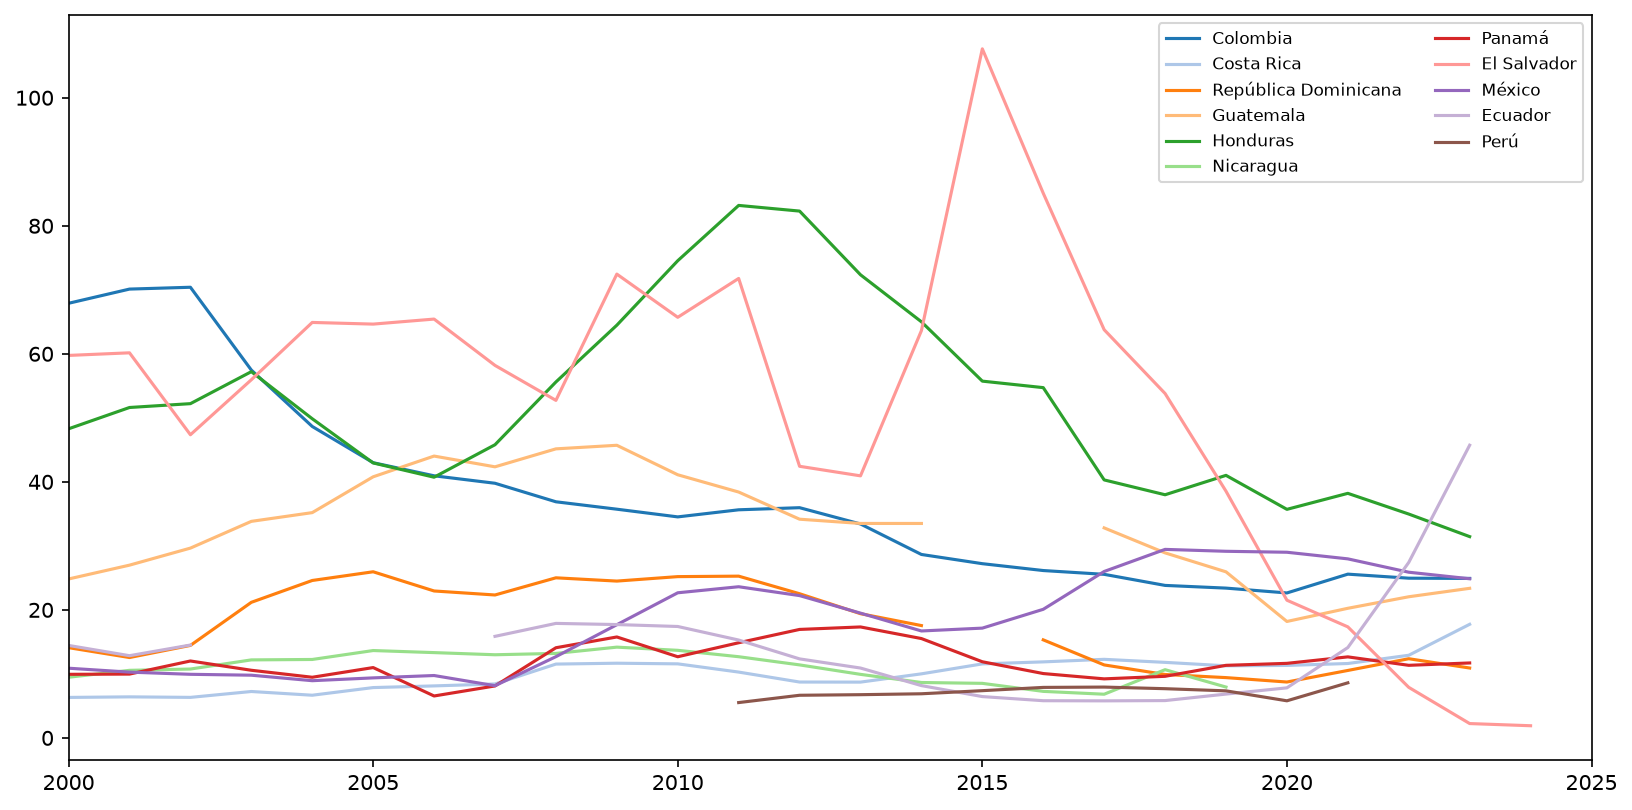
\includegraphics[width=0.73\textwidth]{homicide.png}
    \label{fig:homicidios}
\end{figure}

A partir de este contexto, la presente investigación busca responder la siguiente pregunta de investigación:

\begin{center}
\textit{¿Cómo se relacionan la seguridad, la calidad institucional y el desarrollo económico en Centroamérica, y qué revela el caso de El Salvador sobre dicho mecanismo de transmisión?}
\end{center}

La hipótesis central sostiene que la relación entre seguridad y crecimiento económico es predominantemente indirecta. En particular, se plantea que mayores niveles de violencia deterioran la calidad institucional ---especialmente el Estado de Derecho, el control de la corrupción y la estabilidad política---, reduciendo la capacidad de los países para atraer inversión extranjera y limitando, en consecuencia, su desempeño económico (North, 1990; World Bank, 2011; Acemoglu y Robinson, 2012).

Asimismo, se propone que estos efectos operan en diferentes horizontes temporales. Mientras las condiciones de seguridad pueden modificarse relativamente rápido como consecuencia de cambios en las políticas públicas, las instituciones evolucionan de manera más gradual y los efectos económicos requieren períodos aún mayores para reflejar plenamente dichas transformaciones. Bajo esta perspectiva, el crecimiento económico no respondería de forma inmediata a una reducción de la violencia, sino a través del fortalecimiento progresivo de las instituciones y de un entorno más favorable para la inversión.

La hipótesis central postula un mecanismo secuencial en cuatro etapas:
\[
\underbrace{H_{it}}_{\text{Violencia}}
\;\xrightarrow{\;\beta_1 < 0\;}
\underbrace{Q_{it}}_{\text{Instituciones}}
\;\xrightarrow{\;\gamma_1 > 0\;}
\underbrace{F_{it}}_{\text{IED}}
\;\xrightarrow{\;\delta_1 > 0\;}
\underbrace{G_{it}}_{\text{Crecimiento PIB}}
\]
donde $H$ representa la tasa de homicidios, $Q$ la calidad institucional, $F$ la inversión extranjera directa y $G$ el crecimiento económico. Los signos sobre cada coeficiente indican la dirección esperada de las relaciones planteadas por la hipótesis de investigación.


\section*{Objetivos}
\addcontentsline{toc}{section}{Objetivos}

\subsection*{Objetivo general}

Analizar la relación entre la seguridad, la calidad institucional y el crecimiento económico en Centroamérica mediante un enfoque econométrico de datos de panel, complementado con técnicas de aprendizaje automático, con el propósito de identificar los mecanismos mediante los cuales la seguridad influye en el desempeño económico, tomando a El Salvador como estudio de referencia.
\subsection*{Objetivos específicos}

\begin{enumerate}
    \item Construir una base de datos de panel mediante la extracción, limpieza, integración y transformación de datos provenientes de organismos internacionales, garantizando la consistencia, comparabilidad y calidad de las variables económicas, institucionales y de seguridad utilizadas en el estudio.

    \item Diseñar e implementar un pipeline de análisis que integre técnicas matemáticas, econométricas y de aprendizaje automático para modelar las relaciones entre la seguridad, la calidad institucional y el crecimiento económico, incorporando procedimientos de validación, inferencia robusta y análisis de sensibilidad.

    \item Analizar e interpretar los resultados obtenidos mediante el pipeline, contrastándolos con la teoría de la economía institucional y la evidencia empírica disponible, con el fin de formular conclusiones sobre los mecanismos de transmisión y las diferentes velocidades de ajuste entre seguridad, instituciones y crecimiento económico.
\end{enumerate}

\section{Datos y metodología}

Para analizar esta hipótesis se construyó una base de datos de panel utilizando información proveniente de organismos internacionales de reconocido prestigio. Los indicadores económicos fueron obtenidos del \textit{World Development Indicators} (WDI) del Banco Mundial, los indicadores institucionales de los \textit{Worldwide Governance Indicators} (WGI) y las estadísticas de homicidios de la \textit{United Nations Office on Drugs and Crime} (UNODC).

La base de datos integra información anual para once países de América Latina y el Caribe (los ocho originales de Centroamérica, Colombia y República Dominicana, más México, Ecuador y Perú, incorporados en una extensión posterior del panel dada la relevancia regional de México en materia de seguridad) durante el período 2000--2024, generando un panel de 274 observaciones país-año. El proceso de construcción comprendió un flujo completo de extracción, transformación y carga (ETL), incluyendo la armonización de unidades de medida entre fuentes, tratamiento de valores faltantes, validación de consistencia temporal, generación de variables derivadas y verificación de la estructura del panel antes del análisis econométrico, el dataset, código, documentación y gráficos adicionales se encuentran en:
\begin{center}
\url{https://github.com/mariomarroquin3/data_analyzer}
\end{center}

Las principales variables incluidas fueron:

\begin{itemize}
\item Tasa de homicidios por cada 100\,000 habitantes.
\item Crecimiento anual del PIB.
\item Inversión extranjera directa como porcentaje del PIB.
\item Exportaciones como porcentaje del PIB.
\item Inflación.
\item Desempleo.
\item PIB per cápita (transformado mediante logaritmo natural).
\item Población (transformada mediante logaritmo natural).
\item Llegadas internacionales de turistas (transformadas mediante logaritmo natural).
\item Remesas como porcentaje del PIB (probada como control de robustez; ver Sección~\ref{sec:indice_institucional}).
\item Estado de Derecho (Rule of Law).
\item Control de la Corrupción (Control of Corruption).
\item Estabilidad Política (Political Stability).
\item Voz y Rendición de Cuentas (Voice and Accountability).
\item Efectividad Gubernamental (Government Effectiveness).
\item Calidad Regulatoria (Regulatory Quality).
\end{itemize}

Dado que los seis indicadores institucionales del WGI presentan una elevada correlación y describen dimensiones complementarias de un mismo fenómeno, se construyó un Índice Institucional mediante Análisis de Componentes Principales (Principal Component Analysis, PCA) sobre las seis dimensiones --la construcción estándar en la literatura (Kaufmann et al., 2010), y una ampliación respecto a la versión previa de este estudio, que utilizaba únicamente tres de las seis dimensiones--. Previamente, cada indicador fue estandarizado mediante puntuaciones $z$, garantizando que todos contribuyeran en igualdad de condiciones al índice sintético. El primer componente principal explicó aproximadamente el $72.9\%$ de la variabilidad conjunta, el índice alcanzó un Alfa de Cronbach de $\alpha=0.922$ y una medida de adecuación muestral KMO de $0.863$, indicando una elevada consistencia interna entre las seis dimensiones institucionales consideradas. La Sección~\ref{sec:indice_institucional} discute en detalle por qué esta ampliación de 3 a 6 dimensiones, aunque produce un índice más coherente internamente, cambia de forma material los resultados de las Ecuaciones 1 y 2.

Con el fin de explorar la estructura de correlación entre las variables utilizadas en el análisis, se realizó un análisis exploratorio previo.

\begin{figure}[h]
\centering
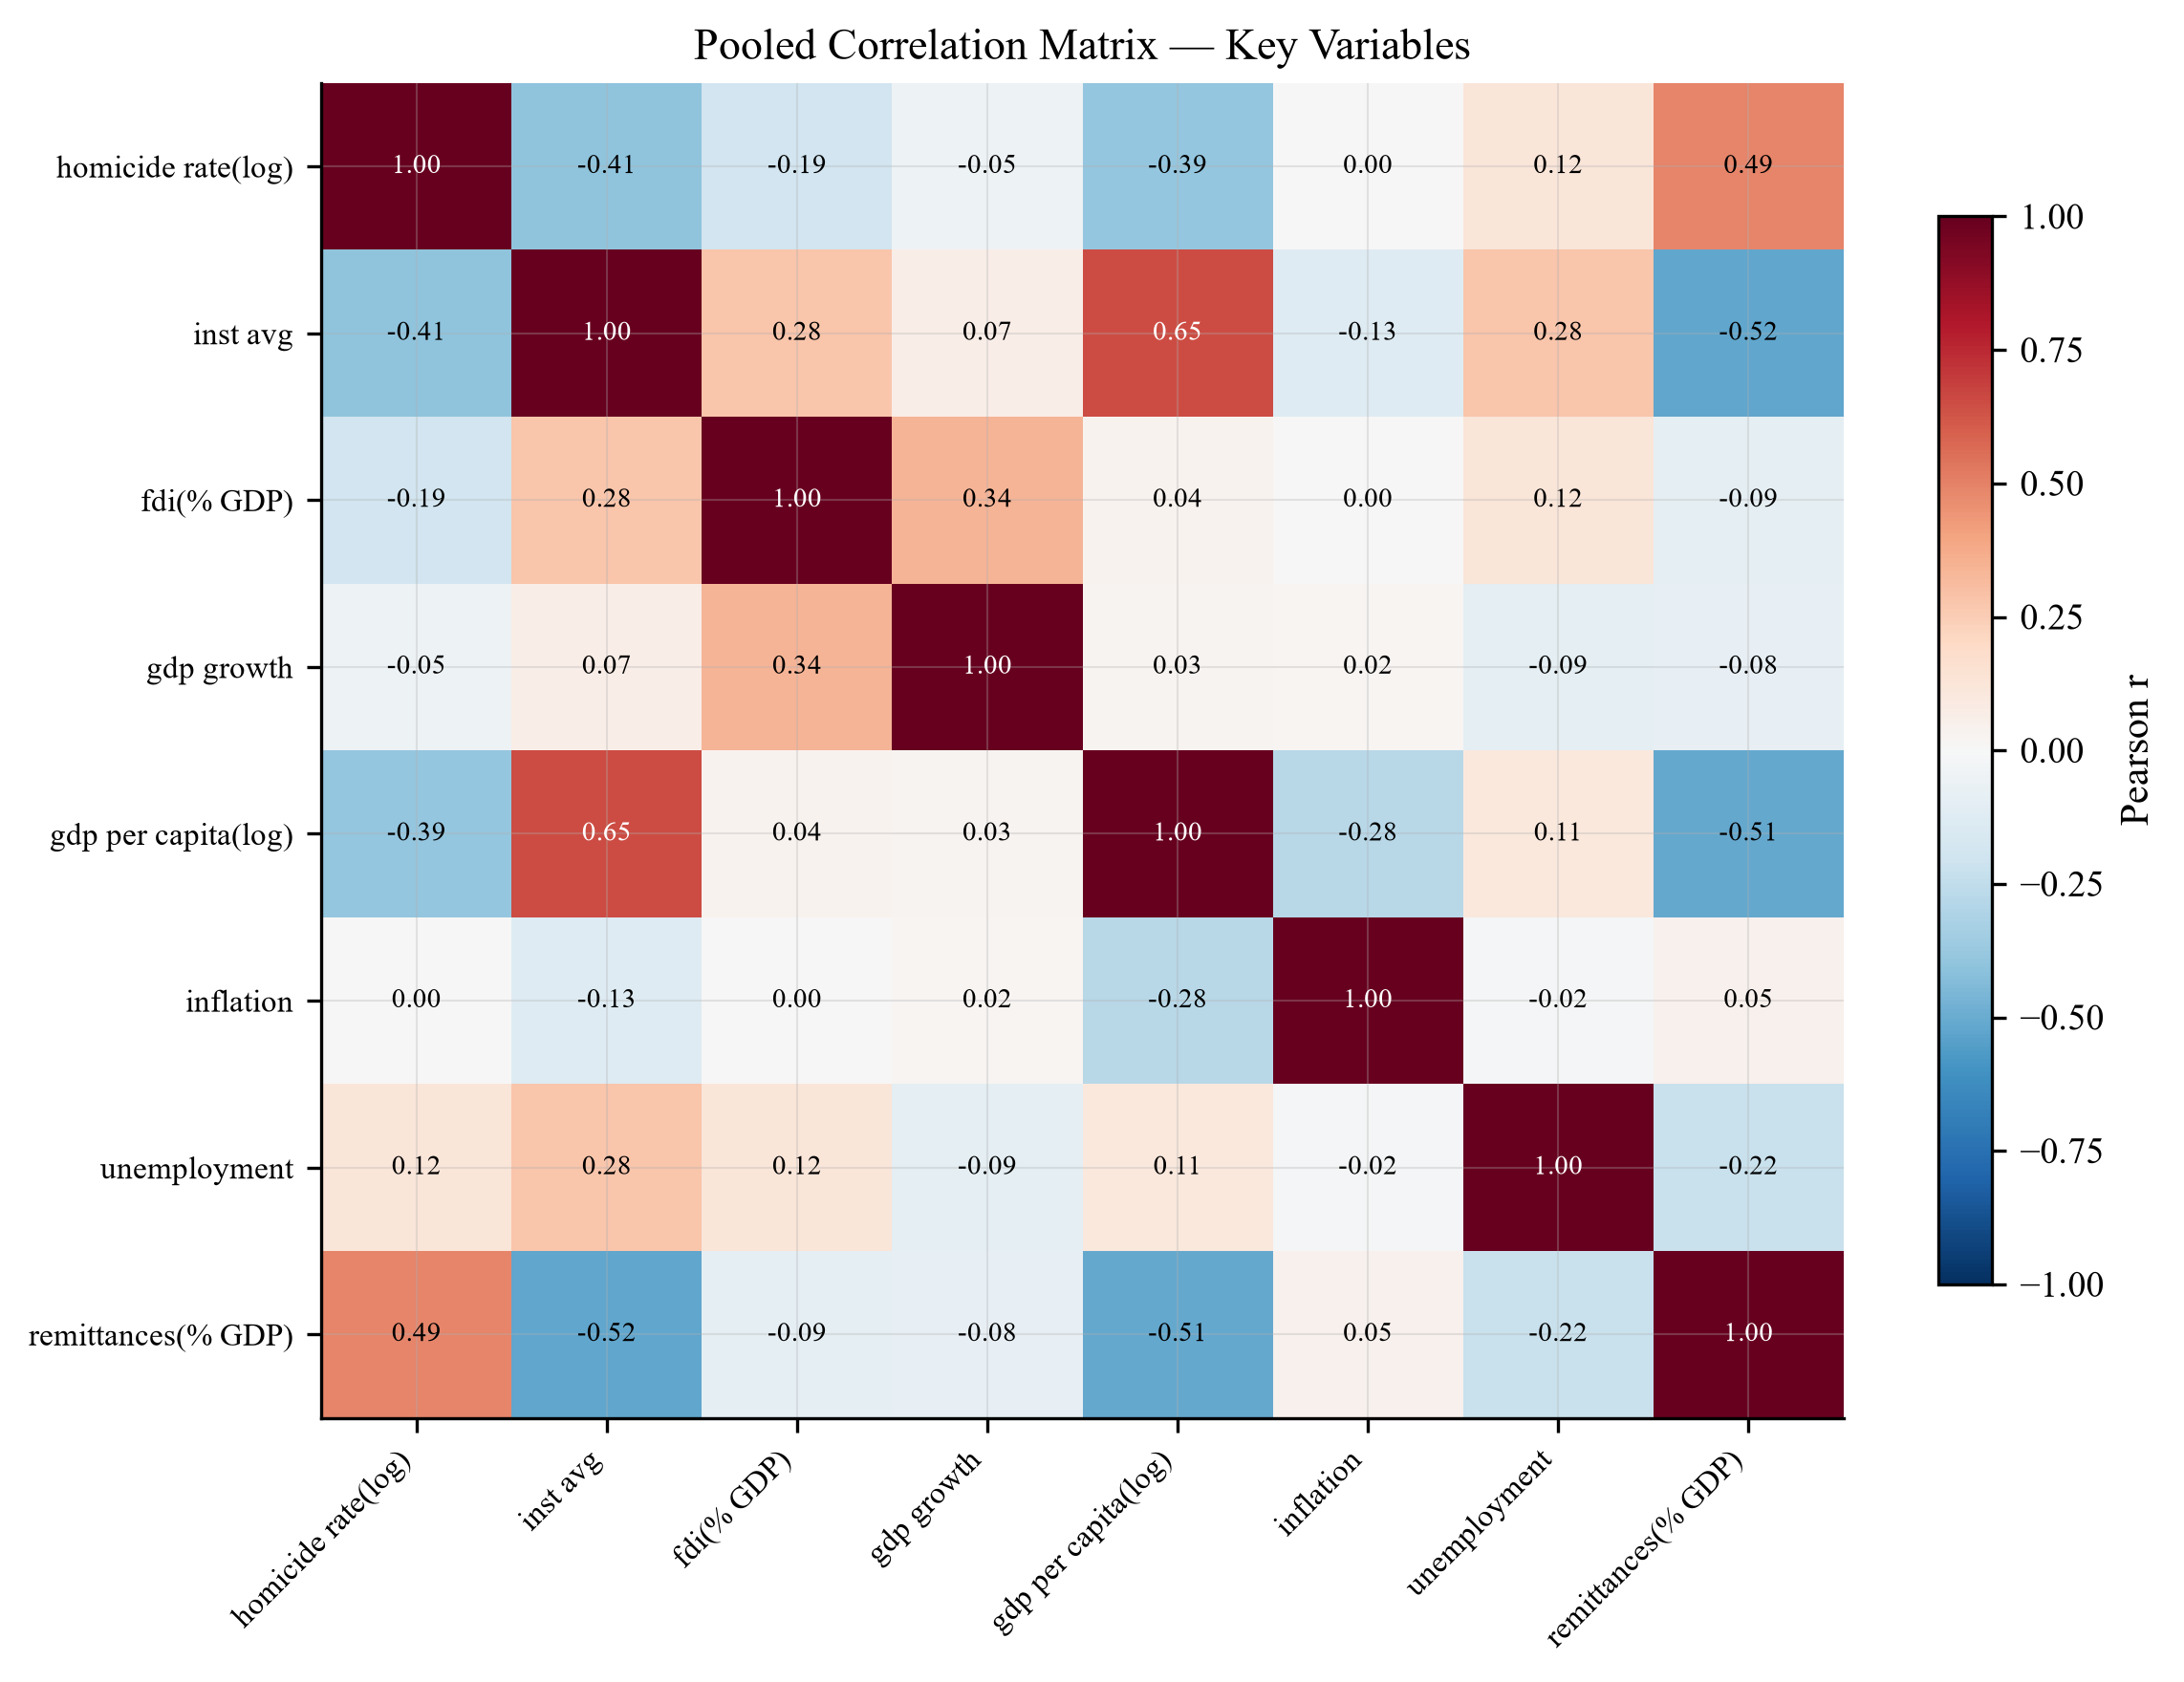
\includegraphics[width=0.85\textwidth]{03_correlation_heatmap.png}
\caption{Matriz de correlación entre variables de seguridad, instituciones y crecimiento económico.}
\label{fig:corr_heatmap}
\end{figure}

El análisis estadístico se desarrolló de manera secuencial. Inicialmente se realizaron análisis descriptivos mediante estadísticas resumen, matrices de correlación y visualizaciones exploratorias. Posteriormente se estimaron modelos de regresión lineal múltiple (OLS) como referencia metodológica. Finalmente, las relaciones principales fueron evaluadas mediante modelos de datos de panel con efectos fijos bidireccionales (\textit{Two-Way Fixed Effects}), incorporando efectos específicos por país y por año para controlar tanto la heterogeneidad no observada entre países como los choques comunes que afectan simultáneamente a toda la región.

Considerando que el panel está compuesto por un número reducido de clústeres (G=11, ampliado desde G=8 en la versión original de este estudio), la inferencia estadística se fortaleció mediante cuatro estimadores de error estándar: errores clusterizados convencionales, errores de Driscoll--Kraay (robustos frente a heterocedasticidad, autocorrelación serial y dependencia transversal), el estimador CR2 de Bell--McCaffrey con grados de libertad de Satterthwaite, y Wild Cluster Bootstrap con pesos de Webb (2023), recomendados para paneles con pocos clústeres. Un coeficiente se describe como ``robusto'' en este documento solo si lo es bajo los cuatro estimadores, no bajo el más favorable de ellos. La estabilidad de las estimaciones fue además evaluada mediante análisis \textit{Leave-One-Country-Out} (LOCO), verificando que los resultados principales permanecieran consistentes al excluir individualmente cada país de la muestra, y mediante un test formal de cointegración de panel para las series no estacionarias de la cadena (Sección~\ref{sec:cointegracion}).

Como complemento al análisis econométrico se implementaron modelos de aprendizaje automático basados en Random Forest Regressor y Gradient Boosting Regressor. Estos modelos no fueron utilizados para establecer relaciones causales, sino para evaluar la importancia relativa de las variables explicativas, detectar posibles relaciones no lineales y contrastar la consistencia de los resultados obtenidos mediante los modelos econométricos tradicionales.

\subsection{Evidencia regional}

El análisis descriptivo muestra que la violencia mantiene una relación estrecha con la calidad institucional de los países analizados. En términos generales, aquellos países que presentan mayores tasas de homicidios también exhiben menores niveles de Estado de Derecho, control de la corrupción y estabilidad política, resultado consistente con la literatura sobre economía institucional.

\begin{figure}[h]
\centering
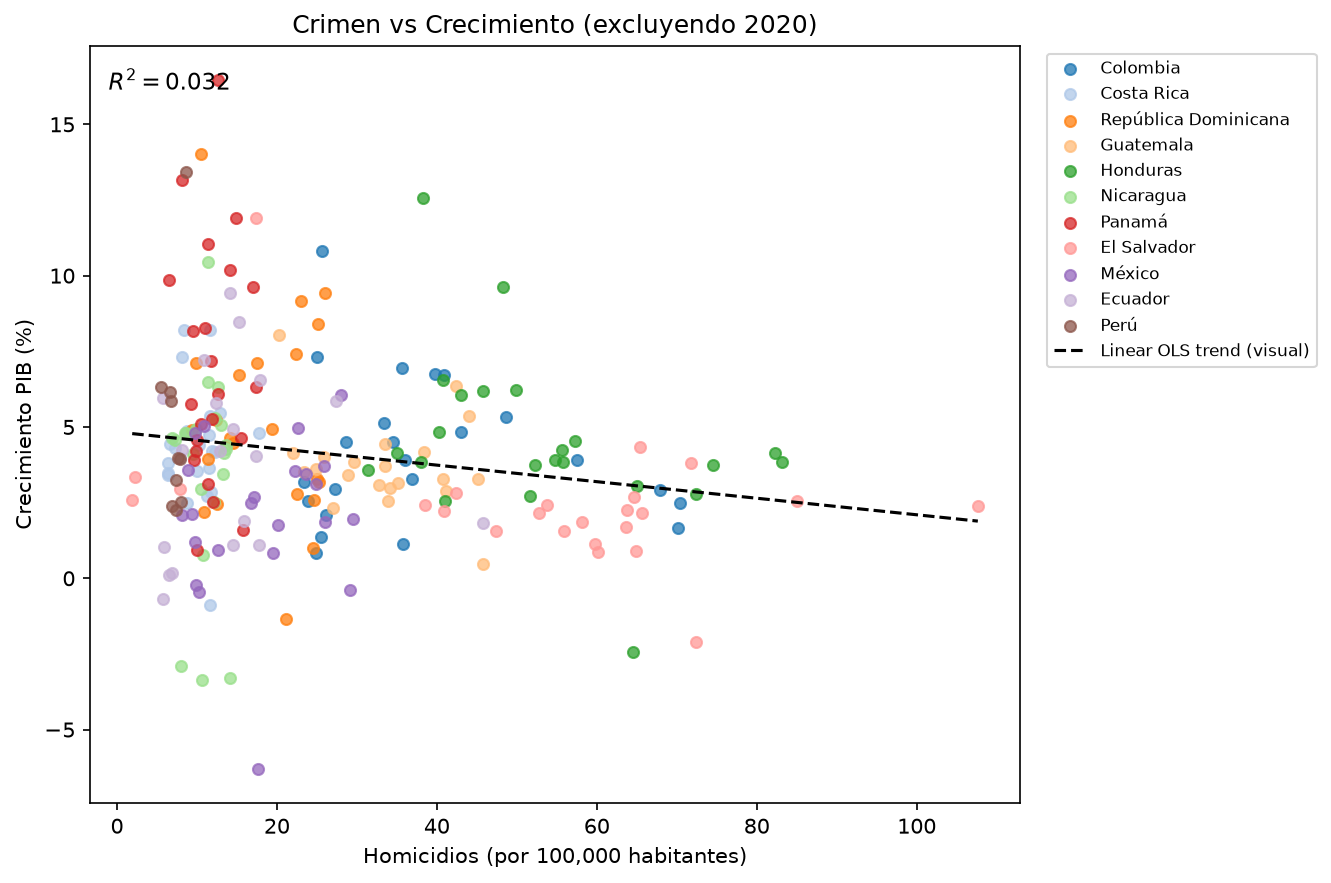
\includegraphics[width=0.79\textwidth]{Figure_2.png}
\caption{Relación entre homicidios y crecimiento económico (excluyendo 2020 por shock exógeno COVID-19).}
\label{fig:crime_growth}
\end{figure}

En contraste, la asociación bivariada entre la violencia y el crecimiento económico resulta débil y heterogénea entre países. El bajo poder explicativo del modelo lineal simple ($R^2 \approx 0.03$ con el panel de once países, frente a $R^2 \approx 0.07$ con el panel original de ocho) sugiere que la relación entre ambas variables no es directa ni estable, sino que está fuertemente condicionada por la heterogeneidad institucional y por mecanismos de transmisión intermedios.

Esta evidencia preliminar respalda la hipótesis central del estudio, según la cual la seguridad no afecta al crecimiento de manera inmediata, sino a través de su impacto sobre la calidad institucional y, posteriormente, sobre la inversión y la acumulación de capital. En este sentido, la ausencia de una relación lineal fuerte no invalida el vínculo teórico, sino que refuerza la necesidad de un enfoque estructural y dinámico del proceso de desarrollo económico.

\subsection{Resultados econométricos principales}

Los modelos de efectos fijos bidireccionales estimados en el pipeline confirman este mecanismo de transmisión en tres etapas:

Las cifras a continuación corresponden a la especificación actual (once países, índice institucional de seis dimensiones). La Sección~\ref{sec:indice_institucional} muestra explícitamente cómo cambian respecto a la versión original de este estudio (ocho países, índice de tres dimensiones).

\textbf{Ecuación 1 (Violencia $\rightarrow$ Instituciones):}

La tasa de homicidios presenta un efecto negativo sobre el índice institucional, pero no significativo bajo ningún estimador:

\[
\beta = -0.0836, \quad p_{\text{cl}} = 0.462, \quad p_{\text{DK}} = 0.310, \quad p_{\text{boot}} = 0.562
\]

El signo es consistente con la teoría institucional, pero la significancia estadística no se alcanza bajo ningún esquema de inferencia. Como se detalla en la Sección~\ref{sec:indice_institucional}, este resultado contrasta con la significancia marginal obtenida bajo el índice institucional de tres dimensiones utilizado en la versión original de este estudio.

\textbf{Ecuación 2 (Instituciones $\rightarrow$ Inversión):}

La calidad institucional tiene un efecto positivo y significativo sobre la inversión extranjera directa en su especificación primaria:

\[
\beta = 0.6111, \quad p_{\text{cl}} = 0.030, \quad p_{\text{DK}} = 0.006, \quad p_{\text{boot}} = 0.038
\]

Este es el eslabón más robusto de la cadena bajo la especificación contemporánea, aunque --a diferencia de lo reportado en la versión original de este estudio-- ya no sobrevive a chequeos de robustez de rezago de un año ($p=0.318$) ni de tendencias específicas por país ($p=0.260$); ver Sección~\ref{sec:indice_institucional}.

\textbf{Ecuación 3 (Inversión + Instituciones $\rightarrow$ Crecimiento):}

La inversión extranjera presenta una asociación positiva y significativa con el crecimiento económico:

\[
\beta_{\text{IED}} = 0.2074, \quad p_{\text{cl}} = 0.010, \quad p_{\text{boot}} = 0.108
\]

El efecto directo de las instituciones sobre el crecimiento, incluido junto con la IED en la misma ecuación, no es significativo ($\beta=-0.544$, $p_{\text{cl}}=0.337$), lo que sugiere que el efecto de las instituciones sobre el crecimiento opera principalmente a través de la IED y no de forma directa.

Un bootstrap formal por clúster de país del efecto indirecto conjunto de la cadena ($\beta_1 \cdot \gamma_1 \cdot \delta_1$) da un punto estimado de $-0.011$ (IC 95\% $=[-0.113, 0.020]$, $p=0.548$): la cadena como sistema mediado único no se rechaza como nula al 5\%, ni bajo la especificación original ni bajo la ampliada.

\subsection{Interpretación estructural del sistema}

En conjunto, los resultados permiten proponer la siguiente cadena de transmisión:

\[
\text{Violencia}
\longrightarrow
\text{Calidad Institucional}
\longrightarrow
\text{Inversión Extranjera Directa}
\longrightarrow
\text{Crecimiento Económico}
\]

Sin embargo, el resultado más importante del pipeline no es únicamente la magnitud de los coeficientes, sino la \textbf{estructura temporal del ajuste económico}.

El alcance temporal de los datos y resultados sugiere que estos procesos no ocurren simultáneamente:

\begin{itemize}
    \item La violencia puede responder relativamente rápido a cambios en las políticas públicas.
    
    \item Las instituciones se ajustan de manera gradual, al depender de procesos acumulativos como el fortalecimiento del Estado de Derecho, la estabilidad política y el control de la corrupción.
    
    \item El desempeño económico puede reaccionar tanto a choques externos de corto plazo como a cambios estructurales de largo plazo. En el contexto de esta investigación, los beneficios derivados de una mejora en la seguridad tienden a manifestarse inicialmente en las empresas ya establecidas, mediante una reducción de los costos asociados a la violencia ---como la extorsión y otros mecanismos de extracción de rentas--- antes de reflejarse en mayores niveles de inversión o crecimiento agregado. La entrada de nueva inversión suele requerir horizontes temporales más largos, debido a los procesos de evaluación, planificación y ejecución propios de los inversionistas.
\end{itemize}

Esta diferencia en velocidades de ajuste explica por qué la relación entre seguridad y crecimiento no es lineal ni contemporánea.

\subsection{Consistencia metodológica del pipeline}

Los resultados son robustos bajo múltiples enfoques:

\begin{itemize}
\item Efectos fijos bidireccionales (país y tiempo).
\item Errores estándar Driscoll--Kraay.
\item Clustering por país (G = 11).
\item Estimador CR2 de Bell--McCaffrey (grados de libertad de Satterthwaite).
\item Wild Cluster Bootstrap (inferencia principal).
\item Leave-One-Country-Out (robustez estructural).
\item Cointegración de panel y modelo de corrección de errores (Sección~\ref{sec:cointegracion}).
\item Modelos de machine learning (Random Forest / Gradient Boosting).
\end{itemize}

En particular, los modelos de aprendizaje automático confirman que las variables institucionales y de violencia se encuentran entre los predictores más importantes del crecimiento económico, aunque sin implicar relaciones lineales estrictas.

En conjunto, el sistema de ecuaciones estimado presenta coherencia en los signos teóricos esperados, aunque con distinta intensidad estadística según la etapa del mecanismo.

\subsection{Validación cruzada Leave-One-Country-Out (LOCO-CV)}

Con el fin de evaluar la estabilidad estructural de las relaciones estimadas, se implementó un procedimiento de validación cruzada tipo Leave-One-Country-Out (LOCO-CV), en el cual cada país es excluido secuencialmente del conjunto de entrenamiento y utilizado como conjunto de prueba. Este enfoque permite analizar la robustez de los modelos ante heterogeneidad transversal y posibles dependencias específicas por país.

\begin{figure}[H]
    \centering
    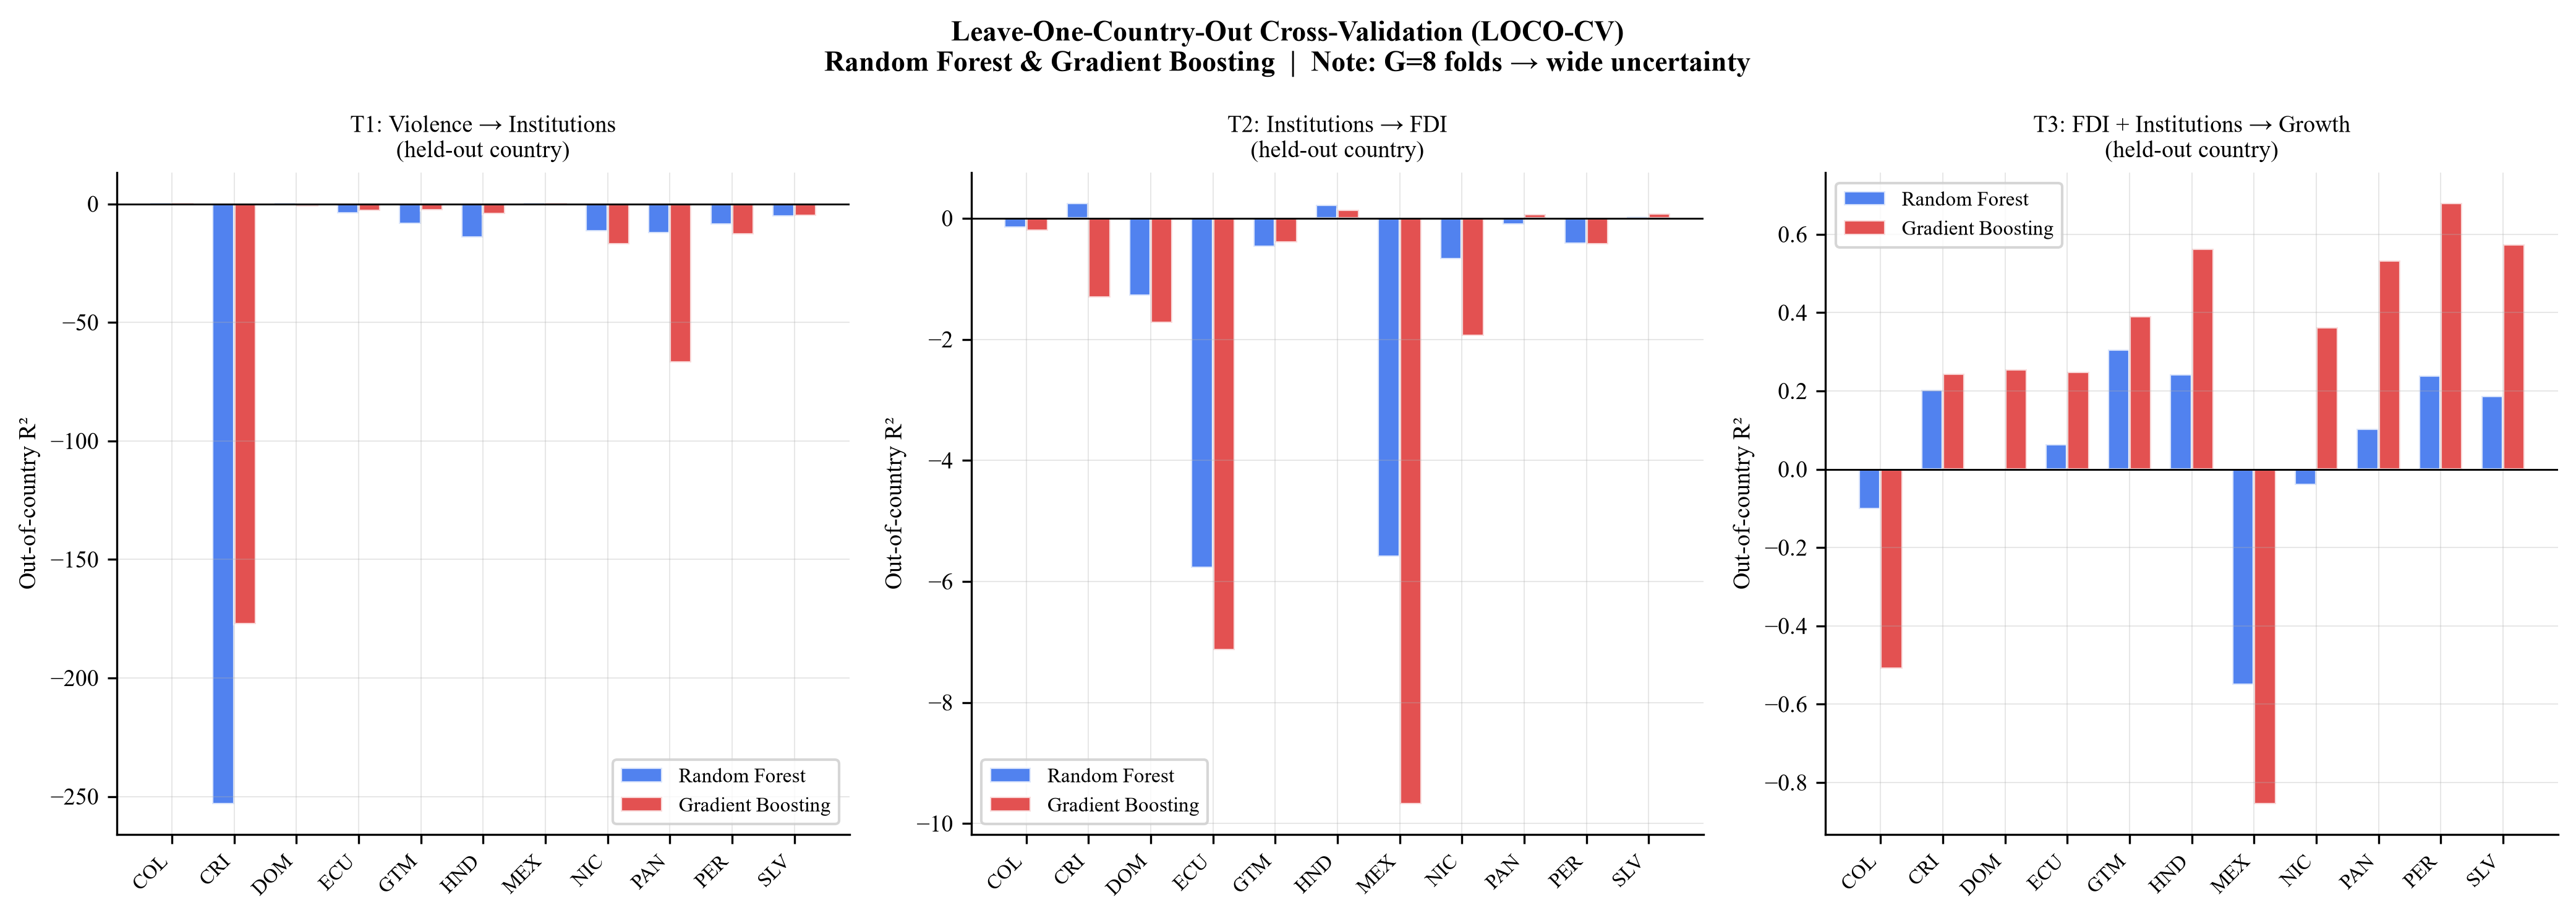
\includegraphics[width=0.95\textwidth]{08_ml_loco_cv.png}
    \caption{Validación cruzada Leave-One-Country-Out (LOCO-CV) para tres relaciones del sistema: (T1) violencia e instituciones, (T2) instituciones e inversión extranjera directa, y (T3) inversión e instituciones sobre crecimiento económico. Se comparan modelos Random Forest y Gradient Boosting.}
    \label{fig:loco_cv}
\end{figure}

Los resultados muestran una elevada heterogeneidad en la capacidad predictiva de los modelos a través de los distintos países. En la relación entre violencia e instituciones (T1), los valores de $R^2$ fuera de muestra son en su mayoría negativos o cercanos a cero, lo que indica una débil capacidad de generalización y una relación estructural inestable entre ambas variables.

De forma similar, la relación entre instituciones e inversión extranjera directa (T2) presenta una alta variabilidad entre países y signos inconsistentes en el desempeño predictivo, lo que sugiere que este vínculo no es homogéneo en la región y depende de características idiosincráticas de cada economía.

En contraste, el modelo que incorpora simultáneamente inversión e instituciones para explicar el crecimiento económico (T3) presenta un desempeño consistentemente superior, especialmente bajo Gradient Boosting, con valores positivos de $R^2$ en la mayoría de los países excluidos. Este resultado sugiere que el crecimiento económico responde mejor a la interacción conjunta de variables institucionales y de inversión, más que a relaciones bivariadas simples.

En conjunto, la evidencia obtenida mediante LOCO-CV refuerza la hipótesis de que el proceso de desarrollo económico opera a través de mecanismos no lineales y con fuertes efectos de heterogeneidad entre países, siendo la etapa final del sistema la que concentra mayor capacidad explicativa fuera de muestra. Este patrón se mantiene con el panel ampliado a once países.

\section{Expansión del Índice Institucional: la Construcción del Índice Importa}
\label{sec:indice_institucional}

La versión original de este estudio construyó el índice institucional a partir de solo tres de las seis dimensiones WGI de Kaufmann et al. (2010) (Estado de Derecho, Control de la Corrupción, Estabilidad Política) --un subconjunto sin justificación metodológica explícita, heredado de un archivo de datos ensamblado manualmente--. Al reconocer esto como una elección arbitraria y no principiada, el índice se reconstruyó utilizando las seis dimensiones, la construcción estándar en la literatura. Los resultados reportados en la Sección~2 utilizan este índice de seis dimensiones.

Las dos especificaciones no son indiferentes entre sí:

\begin{center}
\begin{tabular}{lccc}
\toprule
 & EQ1 (p, clusterizado) & EQ1 (p, Driscoll--Kraay) & EQ2 (p, clusterizado) \\
\midrule
Índice de 3 dimensiones & 0.093 & 0.010 & 0.030 \\
Índice de 6 dimensiones & 0.462 & 0.310 & 0.030 \\
\bottomrule
\end{tabular}
\end{center}

Bajo tres dimensiones, EQ1 era marginalmente significativa bajo tres de los cuatro estimadores. Bajo seis dimensiones --la construcción más completa y estándar-- no lo es bajo ninguno. EQ2 se mantiene significativa en su especificación primaria, pero, como se mencionó en la Sección~2, ya no sobrevive a los chequeos de robustez de rezago ni de tendencias por país que sí superaba bajo el índice de tres dimensiones.

Re-estimar EQ1 con cada una de las seis dimensiones WGI individualmente como variable dependiente (en vez del compuesto) muestra el origen de esta atenuación:

\begin{center}
\begin{tabular}{lcc}
\toprule
Dimensión & Coeficiente & $p$ (clusterizado) \\
\midrule
Estado de Derecho & $-1.961$ & \textbf{0.037} \\
Control de la Corrupción & $-0.395$ & 0.645 \\
Estabilidad Política & $-2.672$ & 0.135 \\
Voz y Rendición de Cuentas & \textbf{+1.721} & 0.339 \\
Efectividad Gubernamental & $-0.999$ & 0.253 \\
Calidad Regulatoria & $-0.277$ & 0.803 \\
\bottomrule
\end{tabular}
\end{center}

Cinco de las seis dimensiones apuntan en la dirección esperada (negativa); Estado de Derecho permanece individualmente significativa. Una dimensión --Voz y Rendición de Cuentas-- apunta en la dirección contraria, con una magnitud suficiente para diluir el promedio compuesto. La Sección~\ref{sec:paradoja_bukele} investiga esta dimensión específicamente y la atribuye a un solo país.

\section{La ``Paradoja Bukele'': Seguridad vs.\ Libertades Civiles}
\label{sec:paradoja_bukele}

Los datos propios de El Salvador explican por qué Voz y Rendición de Cuentas se comporta de forma anómala:

\begin{center}
\begin{tabular}{lcc}
\toprule
Año & Tasa de homicidios (por 100 mil) & Voz y Rendición de Cuentas (0--100) \\
\midrule
2020 & 21.5 & 58.4 \\
2021 & 17.3 & 53.5 \\
2022 & 7.9 & 48.8 \\
2023 & 2.2 & 48.1 \\
2024 & 1.9 & 45.0 \\
\bottomrule
\end{tabular}
\end{center}

De 2021 a 2024 --el período del régimen de excepción-- los homicidios colapsaron \emph{y} Voz y Rendición de Cuentas también cayó. La ganancia de seguridad y el costo en libertades civiles avanzaron juntos, no en direcciones opuestas, justo lo contrario de lo que asume un índice compuesto que trata las seis dimensiones como sustitutos intercambiables de ``calidad institucional''.

Un chequeo Leave-One-Country-Out sobre \texttt{voice\_accountability} $\sim$ \texttt{homicide\_rate\_log\_lag1} (misma especificación de efectos fijos bidireccionales que el resto de EQ1) prueba si esto es un patrón regional o específico de un país:

\begin{center}
\begin{tabular}{lcc}
\toprule
Muestra & Coeficiente & $p$ \\
\midrule
Muestra completa (11 países) & $+1.721$ & 0.339 \\
Excl.\ El Salvador & $\mathbf{-1.482}$ & 0.449 \\
Excl.\ cualquier otro país & $+1.14$ a $+2.74$ (siempre positivo) & -- \\
\bottomrule
\end{tabular}
\end{center}

El Salvador es el \textbf{único} país cuya exclusión invierte el signo. Excluir cualquiera de los otros diez deja el coeficiente positivo; excluir a El Salvador específicamente lo revierte hacia la dirección teóricamente esperada (aunque, con solo diez países restantes, ninguna de las dos estimaciones es en sí misma significativa).

\begin{figure}[H]
\centering
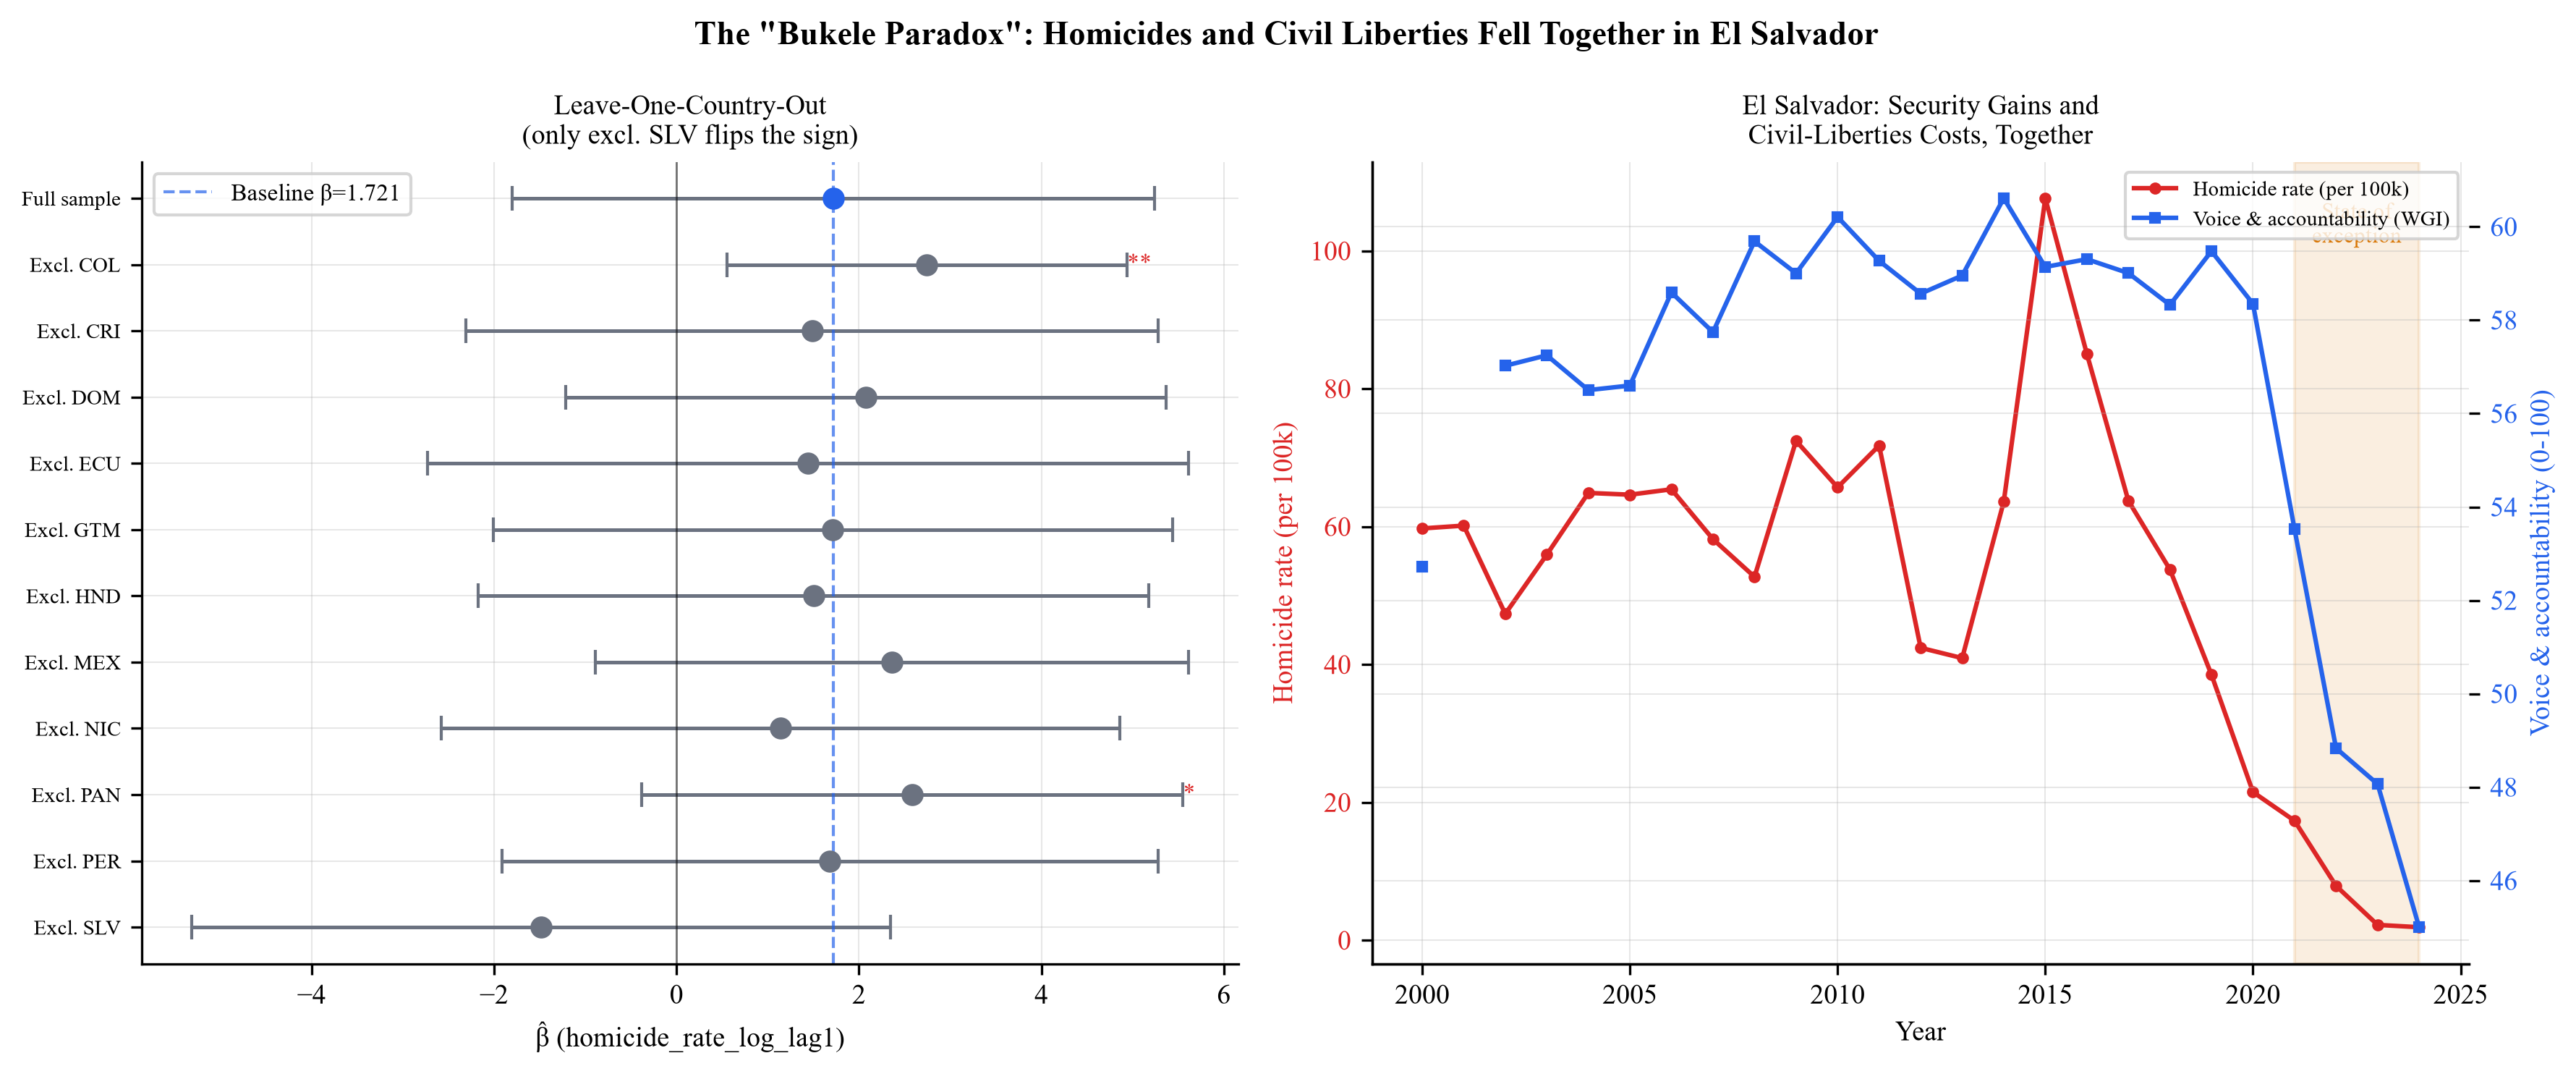
\includegraphics[width=0.95\textwidth]{14_bukele_paradox.png}
\caption{Izquierda: coeficiente LOCO de violencia sobre Voz y Rendición de Cuentas al excluir cada país. Derecha: tasa de homicidios y Voz y Rendición de Cuentas de El Salvador, 2000--2024, con el período del régimen de excepción (2021--2024) resaltado.}
\label{fig:bukele}
\end{figure}

Este hallazgo no se interpreta como un artefacto estadístico a descartar, sino como un hallazgo sustantivo sobre el caso específico de El Salvador, directamente relevante para la pregunta que motiva este estudio. La razón por la que el coeficiente compuesto del índice institucional se diluye bajo la construcción de seis dimensiones no es que la violencia carezca de relación con la calidad institucional --es que una dimensión, en un país, durante una transformación de seguridad específica e históricamente inusual, se movió en dirección opuesta a las otras cinco, porque el rasgo definitorio de esa transformación fue precisamente intercambiar libertades civiles por seguridad.

\section{Cointegración de Panel y Modelo de Corrección de Errores}
\label{sec:cointegracion}

Un test de raíz unitaria de panel (Fisher--ADF, Maddala y Wu, 1999) encuentra que \texttt{homicide\_rate\_log}, \texttt{inst\_avg} y \texttt{gdp\_per\_capita\_log} no rechazan raíz unitaria (son I(1)), mientras que \texttt{fdi\_percent\_gdp} y \texttt{gdp\_growth} sí la rechazan (son I(0)). Dos series I(1) pueden compartir una relación de equilibrio de largo plazo genuina (cointegración), en cuyo caso una regresión estática en niveles no sería necesariamente espuria. Se prueba esto mediante el enfoque de dos pasos de Engle--Granger extendido a panel (Kao, 1999; McCoskey y Kao, 1998) para los tres pares de variables I(1) del panel.

\begin{center}
\begin{tabular}{lccc}
\toprule
Par & $\beta$ (largo plazo) & $p$ (Fisher, residuos) & ¿Cointegrado? \\
\midrule
T1: Homicidios $\leftrightarrow$ Instituciones & $-0.133$ & 0.636 & No \\
T2: Instituciones $\leftrightarrow$ Ingreso & $0.773$ & 0.393 & No \\
T3: Homicidios $\leftrightarrow$ Ingreso & $-0.091$ & \textbf{0.011} & \textbf{Sí} \\
\bottomrule
\end{tabular}
\end{center}

Para T3, el modelo de corrección de errores encuentra $\varphi=-0.109$ ($p=0.006$ clusterizado, $p<0.001$ Driscoll--Kraay): el PIB per cápita corrige aproximadamente el 11\% de cualquier desviación de su relación de largo plazo con la violencia cada año --el primer resultado dinámico, no solo estático, de este estudio--. El efecto de corto plazo ($\gamma=-0.033$, $p=0.344$) no es significativo; solo el ajuste de largo plazo lo es. T1 y T2 no muestran evidencia de cointegración, consistente con (y ofreciendo una explicación formal adicional para) la inestabilidad de EQ1 en cada otro chequeo de este estudio.

\begin{figure}[H]
\centering
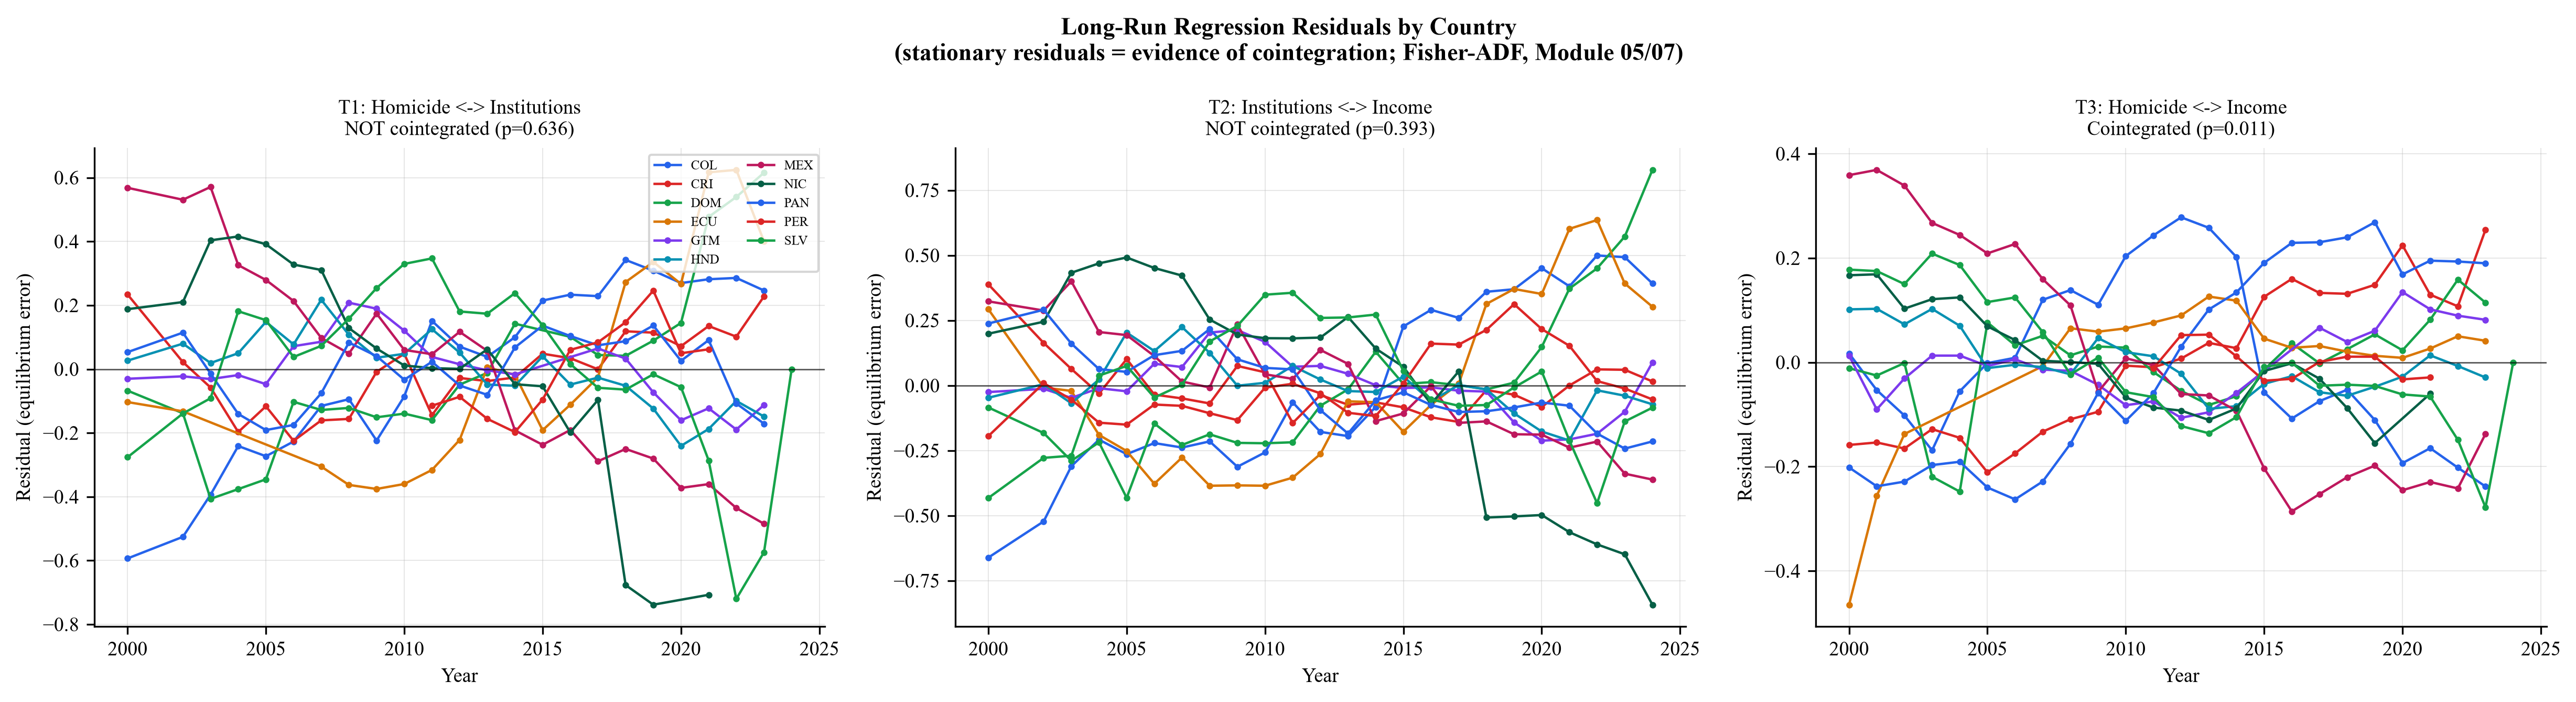
\includegraphics[width=0.95\textwidth]{11_cointegration_residuals.png}
\caption{Residuos de la regresión de largo plazo por país para los tres pares I(1). Residuos estacionarios (T3) son evidencia de cointegración; residuos que se alejan persistentemente (T1, T2) son evidencia de una relación potencialmente espuria.}
\label{fig:cointegration}
\end{figure}

\section{Growth-Ceiling-at-Risk: una Exploración Bayesiana}
\label{sec:growth_ceiling}

Una regresión cuantílica exploratoria de \texttt{gdp\_growth} sobre violencia rezagada (cuantiles 0.05--0.95) encontró que la violencia no tiene efecto cerca de la mediana de la distribución de crecimiento, pero sí un efecto negativo grande y robusto a LOCO en la cola \emph{superior} (q=0.90/0.95) --el reflejo especular del Growth-at-Risk clásico (Adrian, Boyarchenko y Giannone, 2019), que estudia la cola inferior--. Alta violencia no empeora los años malos; limita cuánto puede crecer un año bueno.

Este patrón se re-estimó como una regresión cuantílica bayesiana jerárquica (verosimilitud Asimétrica de Laplace; Yu y Moyeed, 2001) con partial pooling entre los once países (parametrización no centrada; Betancourt y Girolami, 2015) en lugar de variables dummy por país, apuntando a la distribución posterior completa en cada cuantil:

\begin{center}
\begin{tabular}{lcccc}
\toprule
Cuantil ($\tau$) & Coef.\ frecuentista & Media posterior & 94\% HDI & $P(\beta<0\mid\text{datos})$ \\
\midrule
0.50 (mediana) & $-0.08$ ($p=0.827$) & $-0.23$ & $[-0.77, 0.37]$ & 0.790 \\
0.90 & $-2.23$ ($p=0.0005$) & $\mathbf{-1.76}$ & $\mathbf{[-2.93,-0.59]}$ & \textbf{0.997} \\
0.95 & $-2.06$ ($p=0.0043$) & $\mathbf{-2.08}$ & $\mathbf{[-3.02,-1.11]}$ & \textbf{1.000} \\
\bottomrule
\end{tabular}
\end{center}

Los diagnósticos de MCMC son limpios en cada cuantil (R-hat $\leq 1.004$, tamaño de muestra efectivo $>1{,}100$, cero divergencias en 4 cadenas $\times$ 1{,}000 muestras post-calentamiento). Un chequeo secundario con \texttt{inst\_avg} en lugar de violencia no encuentra efecto de techo (prácticamente un volado, $P(\beta<0)=0.367$ y $0.597$) --el efecto es específico a la violencia--.

\begin{figure}[H]
\centering
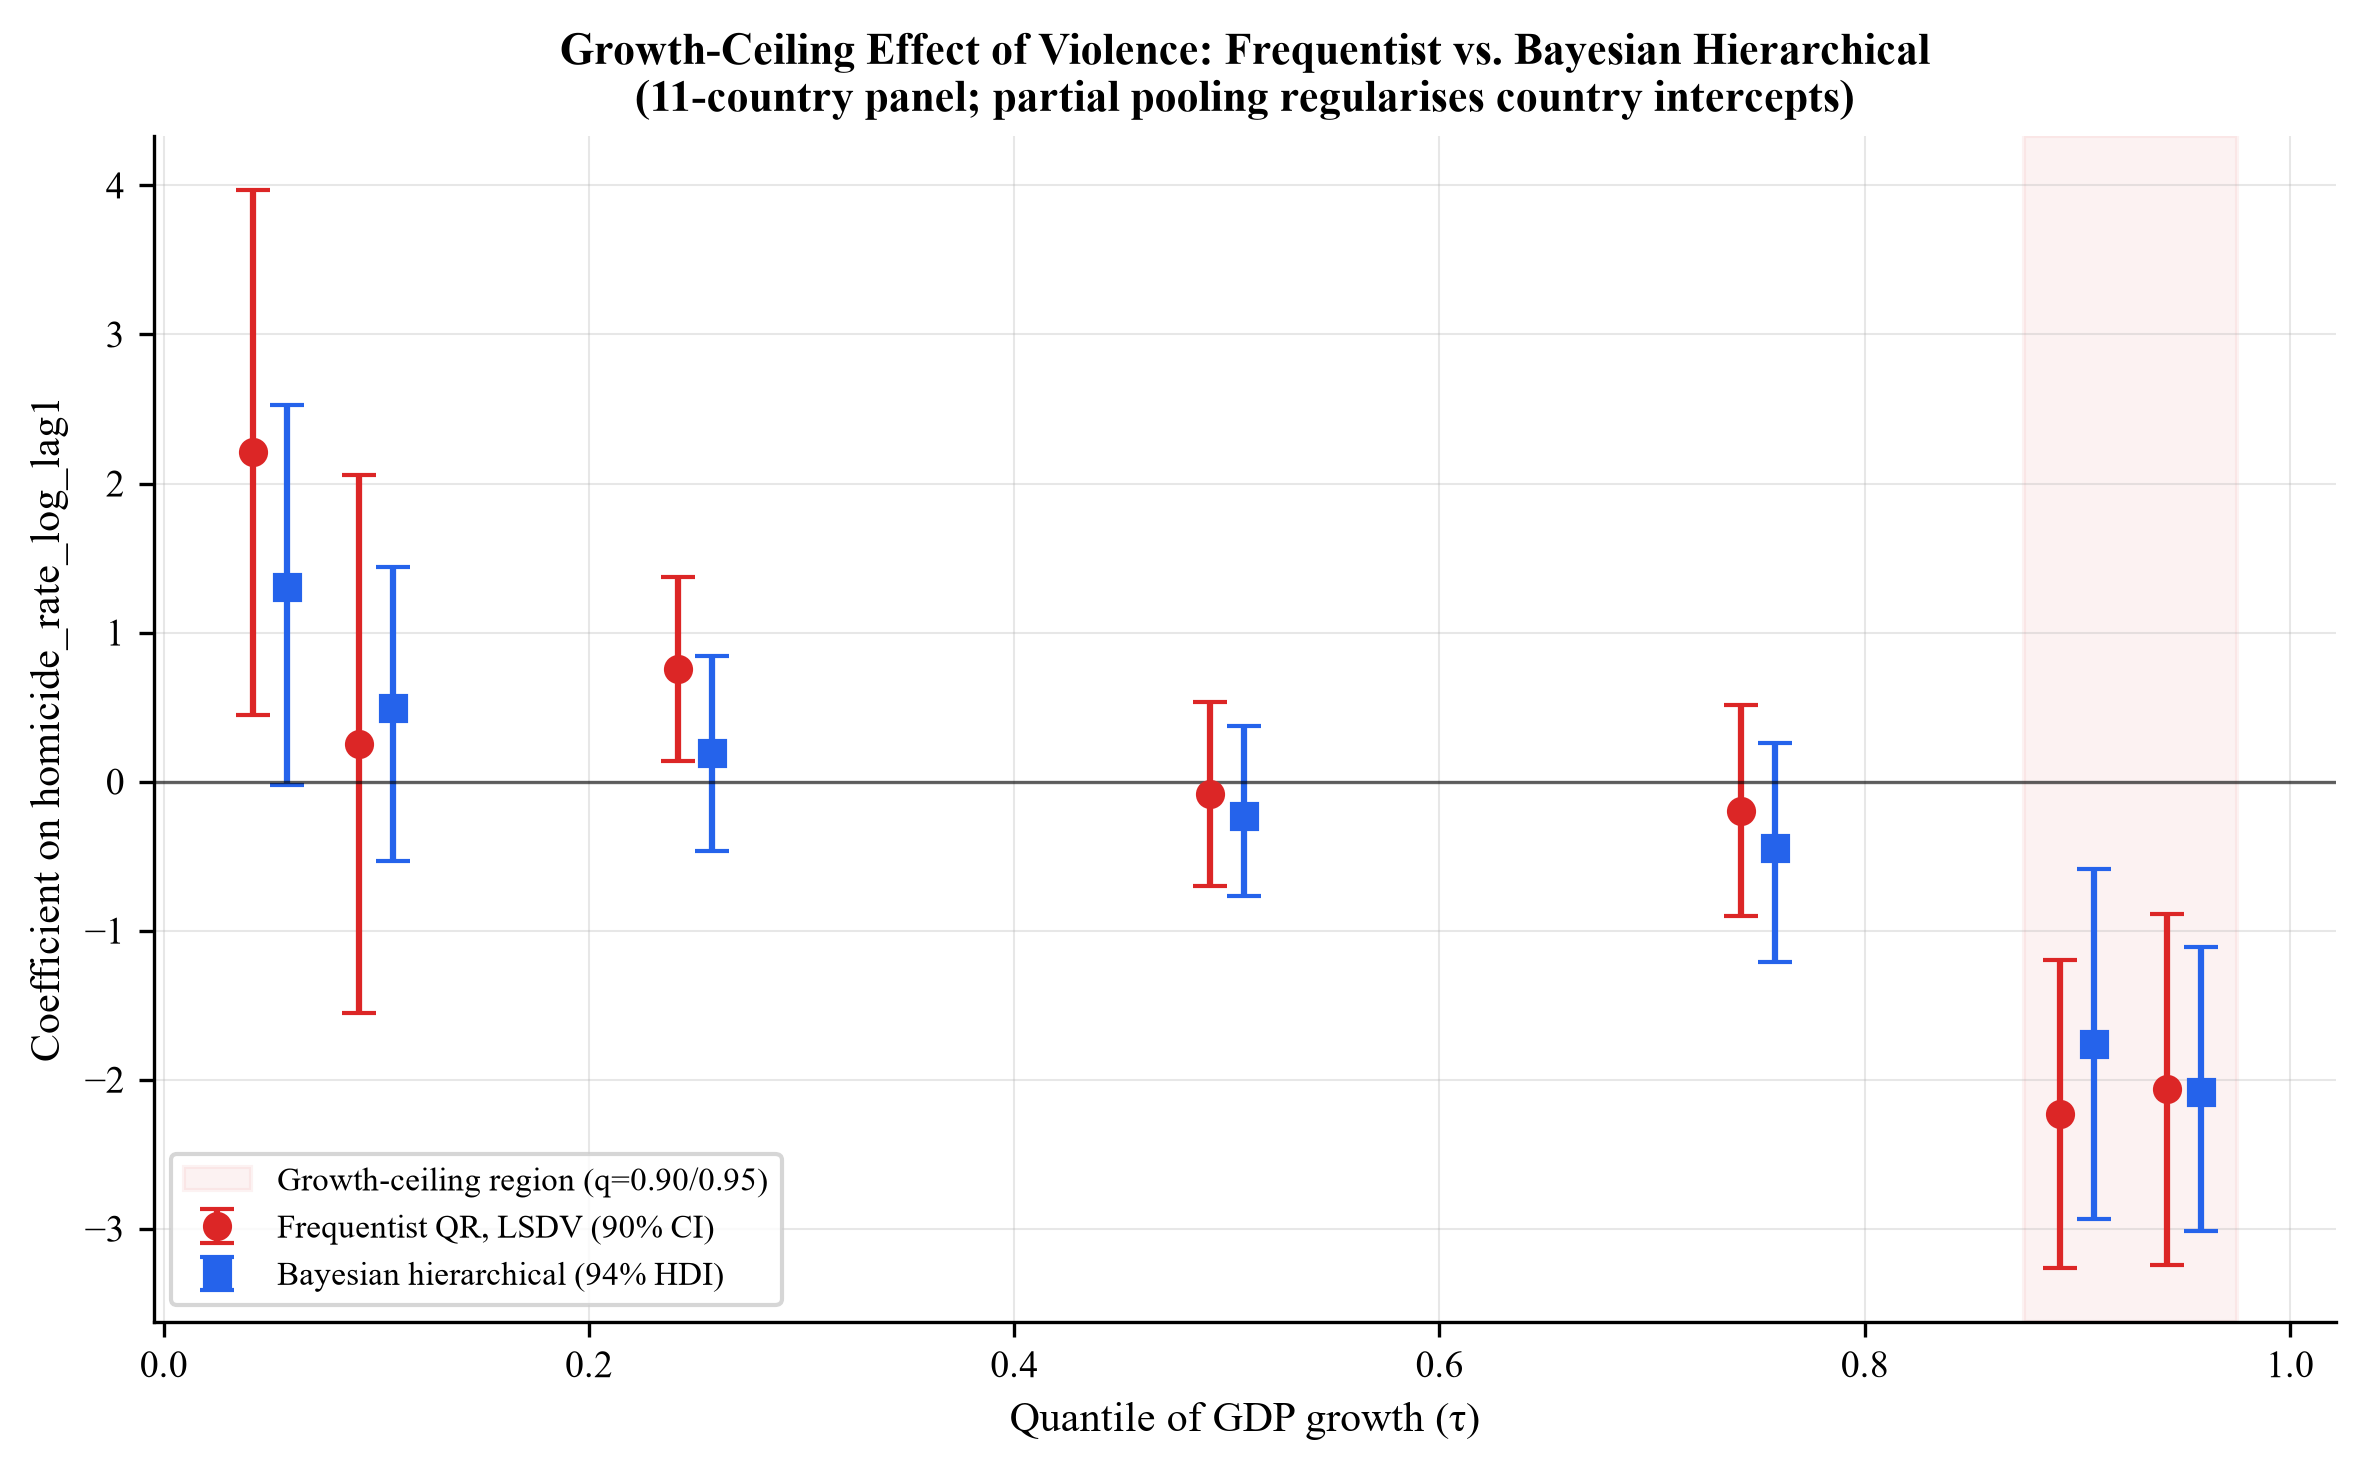
\includegraphics[width=0.95\textwidth]{12_growth_ceiling_bayesian.png}
\caption{Coeficiente de violencia por cuantil del crecimiento del PIB, frecuentista vs.\ bayesiano jerárquico.}
\label{fig:gcar_coef}
\end{figure}

Manteniendo país y año en su nivel promedio, la posterior responde directamente la pregunta aplicada: ¿cuánto baja el techo de crecimiento alcanzable cuando la violencia rezagada pasa de su percentil 10 al percentil 90?

\begin{center}
\begin{tabular}{lccc}
\toprule
Cuantil & Techo (violencia baja) & Techo (violencia alta) & Caída \\
\midrule
0.90 & 8.79 pts & 5.52 pts & 3.27 pts ($P(\text{caída}>0)=0.997$) \\
0.95 & 10.29 pts & 6.43 pts & 3.86 pts ($P(\text{caída}>0)>0.999$) \\
\bottomrule
\end{tabular}
\end{center}

\begin{figure}[H]
\centering
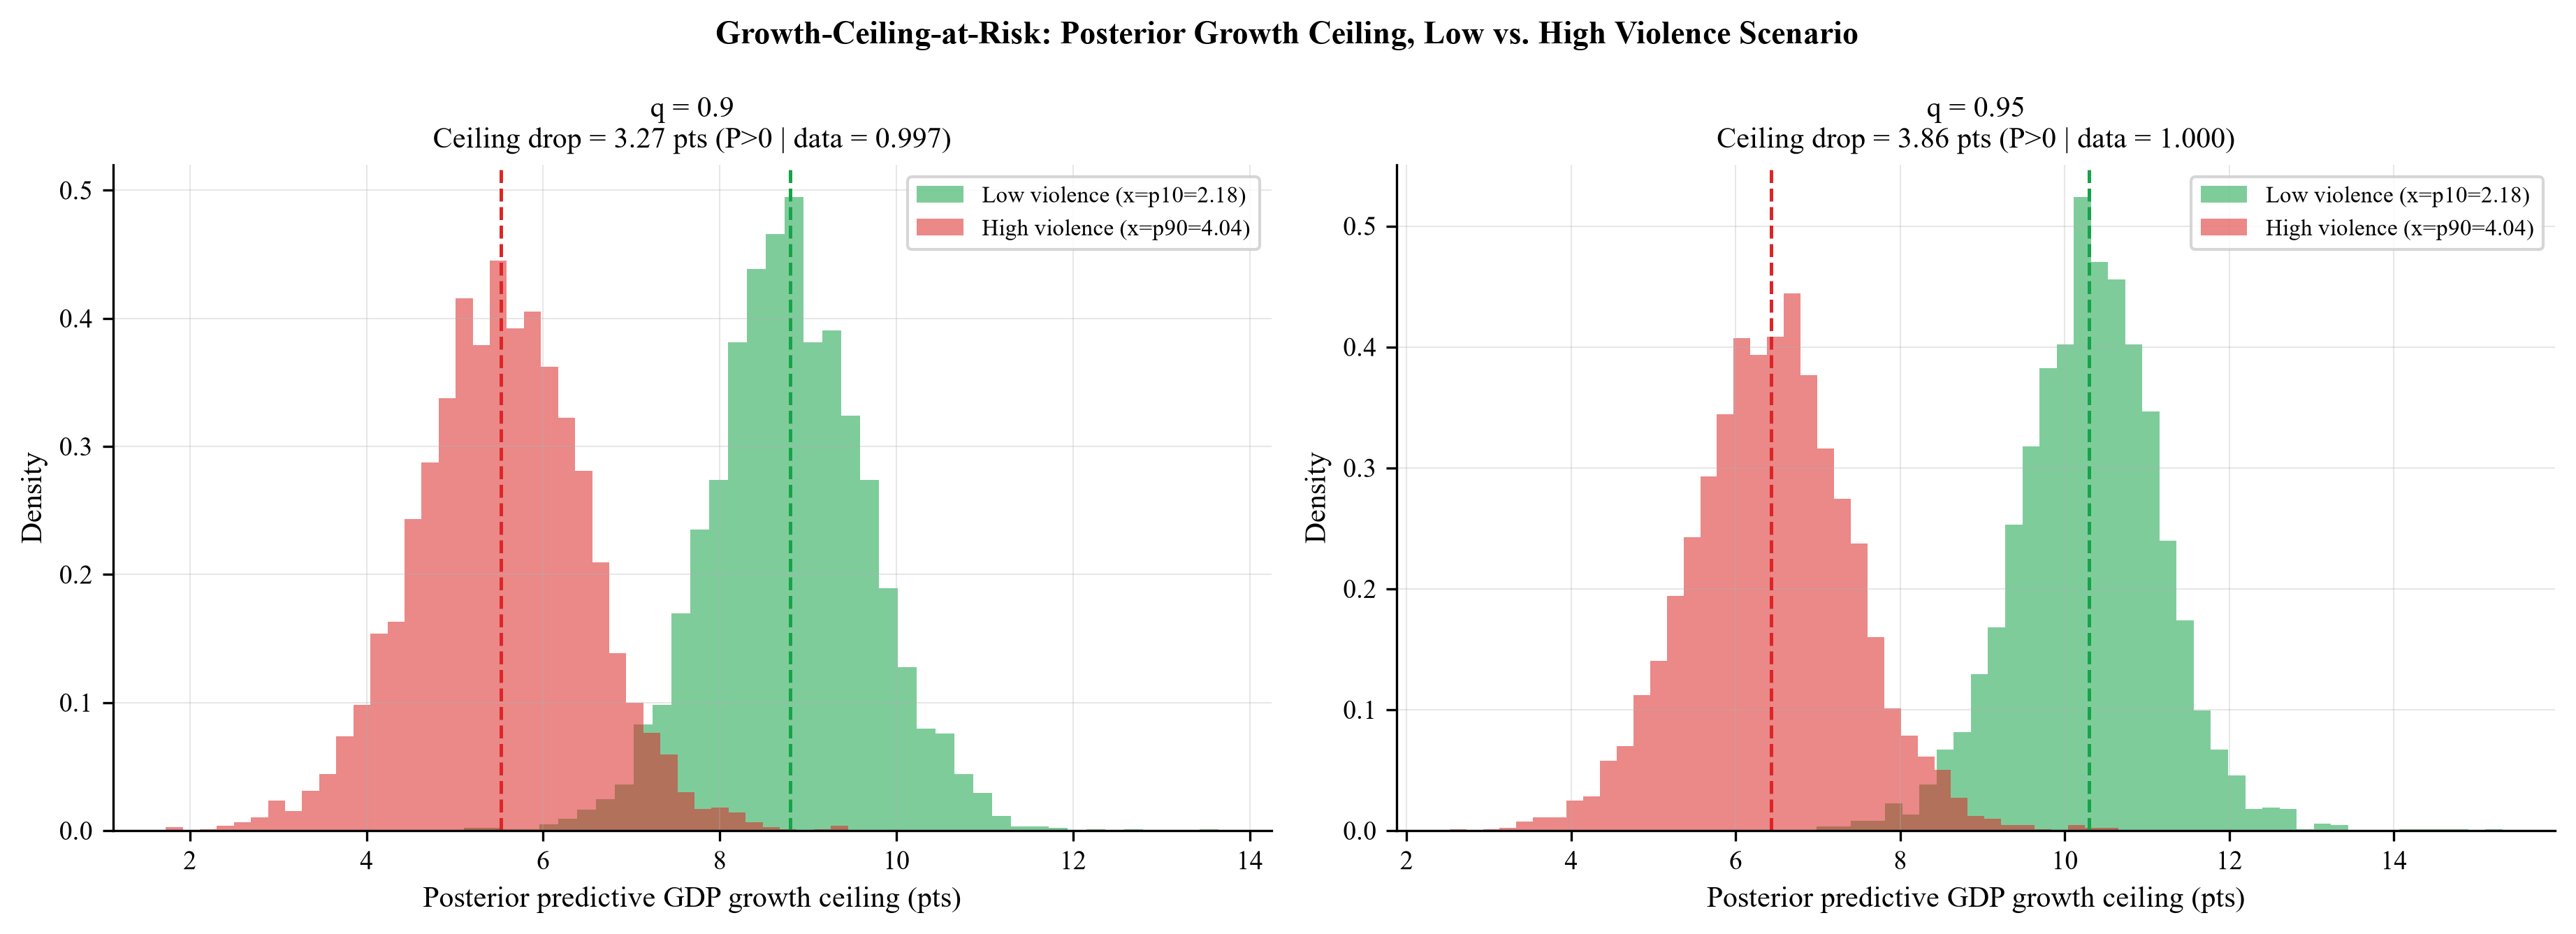
\includegraphics[width=0.85\textwidth]{13_growth_ceiling_scenario.png}
\caption{Distribución posterior del techo de crecimiento bajo escenarios de violencia baja (percentil 10) vs.\ alta (percentil 90).}
\label{fig:gcar_scenario}
\end{figure}

Este es un hallazgo exploratorio --motivado por un patrón encontrado post-hoc, no por una hipótesis pre-registrada--. G=11 sigue siendo pequeño incluso para un modelo jerárquico, y el hallazgo central es precisamente que el efecto NO es monótono: nulo en la mediana, negativo solo en la cola superior.

\section*{Conclusiones}
\addcontentsline{toc}{section}{Conclusiones}

Los resultados muestran que la reducción de la violencia, por sí sola, no se traduce necesariamente en un incremento inmediato del crecimiento económico. El resumen honesto de este estudio, ampliado a once países y con un índice institucional completo de seis dimensiones, no es ``la violencia deteriora las instituciones, lo cual reduce la IED y el crecimiento'': los datos, estimados con rigor y reportados en su totalidad en vez de seleccionando el resultado más favorable, no respaldan una historia tan limpia. Lo que los datos sí respaldan es más acotado y, creemos, más útil: instituciones $\rightarrow$ IED es el eslabón más defendible del panel; violencia $\rightarrow$ instituciones es frágil y depende de la especificación --significativa bajo una construcción arbitraria de tres dimensiones del índice, no significativa bajo la construcción estándar de seis--; y donde la relación agregada resulta anómala (una dimensión de gobernanza que se mueve en la dirección ``equivocada''), descomponerla revela una explicación específica e interpretable a nivel de caso (el deterioro de voz y rendición de cuentas en El Salvador) en vez de ruido sin explicar. El bajo poder explicativo del modelo bivariado entre homicidios y crecimiento ($R^2 \approx 0.03$ con once países) refuerza la idea de ausencia de una relación contemporánea estable.

El principal aporte de esta investigación consiste en proponer una interpretación dinámica de este proceso. Más que considerar la seguridad, las instituciones y el crecimiento como variables que evolucionan simultáneamente, la evidencia indica que cada una responde en horizontes temporales diferentes.

Las condiciones de seguridad pueden modificarse relativamente rápido como consecuencia de cambios en las políticas públicas. En contraste, las instituciones reflejan procesos acumulativos asociados al fortalecimiento del Estado de Derecho, la estabilidad política y el control de la corrupción, cuya consolidación requiere períodos considerablemente más largos. Finalmente, las variables macroeconómicas incorporan estos cambios de manera gradual, conforme hogares, empresas e inversionistas ajustan sus decisiones.

Desde esta perspectiva, la ausencia de una relación contemporánea fuerte entre violencia y crecimiento económico no contradice la teoría institucional. Por el contrario, resulta consistente con un sistema en el que los efectos económicos aparecen con rezago debido a que las distintas dimensiones del desarrollo evolucionan a velocidades diferentes.

En conjunto, la evidencia obtenida invita a interpretar la seguridad no únicamente como un determinante aislado del crecimiento, sino como una manifestación observable de la capacidad institucional del Estado. Desde esta perspectiva, una reducción sostenida de la violencia refleja la consolidación del monopolio de la fuerza y una disminución de los costos de transacción y de cumplimiento que enfrentan los agentes económicos. Sin embargo, los beneficios macroeconómicos de este proceso no se materializan de forma instantánea, sino que operan a diferentes velocidades de ajuste.

El caso de El Salvador ilustra con claridad esta dinámica asincrónica. La rápida contracción de la criminalidad constituye un cambio estructural inmediato en las condiciones de seguridad; no obstante, sus efectos económicos iniciales tienden a manifestarse a nivel microeconómico, a través de ajustes en los costos operativos del tejido empresarial existente y del amplio sector informal. Esto es consistente con la teoría institucional, en la que la reducción de dinámicas de extorsión y extracción de rentas genera una mejora inmediata en los costos de producción, antes de que estos efectos se reflejen plenamente en la inversión agregada o en el crecimiento.

En términos generales, los resultados no solo permiten contrastar la hipótesis planteada, sino también proponer un marco interpretativo en el que la seguridad, las instituciones y el crecimiento deben entenderse como un sistema dinámico con rezagos heterogéneos. Bajo esta interpretación, la ausencia de efectos inmediatos no implica ausencia de causalidad, sino diferencias en la velocidad de transmisión del impacto económico.

Comprender estas diferencias en los tiempos de respuesta resulta fundamental para la evaluación de políticas públicas. Concluir prematuramente que la ausencia de crecimiento inmediato implica la inexistencia de efectos económicos positivos significaría ignorar que la seguridad constituye una condición necesaria, pero de maduración lenta, cuyo impacto se materializa únicamente a través del fortalecimiento progresivo de las instituciones productivas y de la posterior respuesta de la inversión y la actividad económica.

Las extensiones metodológicas de esta versión refuerzan, más que socavan, esta interpretación dinámica. El test de cointegración de panel (Sección~\ref{sec:cointegracion}) encuentra una relación de equilibrio de largo plazo genuina entre violencia e ingreso, con el PIB per cápita corrigiendo cerca del 11\% de cualquier desviación cada año --un resultado dinámico que la especificación estática original no podía producir--. Y un patrón exploratorio pero robusto a LOCO --la violencia comprime la cola superior del crecimiento alcanzable sin afectar su mediana (Sección~\ref{sec:growth_ceiling})-- motiva una dirección específica y falsable para trabajo futuro. Finalmente, el caso de El Salvador --el motivo original de este estudio-- resultó ser no solo el caso que ilustra la dinámica asincrónica entre seguridad e instituciones, sino también el único país cuya trayectoria reciente explica por qué una de las seis dimensiones de calidad institucional se comporta de forma anómala en el panel: las ganancias de seguridad y el deterioro de las libertades civiles avanzaron juntos, no en direcciones opuestas, durante su transformación de seguridad.
\section*{Bibliografía}
\addcontentsline{toc}{section}{Bibliografía}

Acemoglu, D. and Robinson, J.A. (2012) \textit{Why Nations Fail: The Origins of Power, Prosperity, and Poverty}. New York: Crown Business.

Adrian, T., Boyarchenko, N. and Giannone, D. (2019) 'Vulnerable Growth', \textit{American Economic Review}, 109(4), pp. 1263--1289.

Angrist, J.D. and Pischke, J.-S. (2009) \textit{Mostly Harmless Econometrics: An Empiricist's Companion}. Princeton: Princeton University Press.

Betancourt, M. and Girolami, M. (2015) 'Hamiltonian Monte Carlo for hierarchical models', in \textit{Current Trends in Bayesian Methodology with Applications}.

Besley, T. and Persson, T. (2011) \textit{Pillars of Prosperity: The Political Economics of Development Clusters}. Princeton: Princeton University Press.

Breiman, L. (2001) 'Random forests', \textit{Machine Learning}, 45(1), pp. 5--32.

Cameron, A.C. and Miller, D.L. (2015) 'A practitioner's guide to cluster-robust inference', \textit{Journal of Human Resources}, 50(2), pp. 317--372.

Diario El Mundo (2024) 'El Salvador con cerca del 70\% de empleo informal, una de las tasas más altas de América Latina'. Disponible en: \url{https://diario.elmundo.sv/economia/el-salvador-con-cerca-del-70-de-empleo-informal-una-de-las-tasas-mas-altas-de-america-latina}

Driscoll, J.C. and Kraay, A.C. (1998) 'Consistent covariance matrix estimation with spatially dependent panel data', \textit{Review of Economics and Statistics}, 80(4), pp. 549--560.

Engle, R.F. and Granger, C.W.J. (1987) 'Co-integration and error correction: representation, estimation, and testing', \textit{Econometrica}, 55(2), pp. 251--276.

Gelman, A. and Hill, J. (2007) \textit{Data Analysis Using Regression and Multilevel/Hierarchical Models}. Cambridge: Cambridge University Press.

Kao, C. (1999) 'Spurious regression and residual-based tests for cointegration in panel data', \textit{Journal of Econometrics}, 90(1), pp. 1--44.

Kaufmann, D., Kraay, A. and Mastruzzi, M. (2010) \textit{The Worldwide Governance Indicators: Methodology and Analytical Issues}. World Bank Policy Research Working Paper No. 5430.

Maddala, G.S. and Wu, S. (1999) 'A comparative study of unit root tests with panel data and a new simple test', \textit{Oxford Bulletin of Economics and Statistics}, 61(S1), pp. 631--652.

McCoskey, S. and Kao, C. (1998) 'A residual-based test of the null of cointegration in panel data', \textit{Econometric Reviews}, 17(1), pp. 57--84.

North, D.C. (1990) \textit{Institutions, Institutional Change and Economic Performance}. Cambridge: Cambridge University Press.

Rodrik, D., Subramanian, A. and Trebbi, F. (2004) 'Institutions rule: The primacy of institutions over geography and integration in economic development', \textit{Journal of Economic Growth}, 9(2), pp. 131--165.

United Nations Office on Drugs and Crime (2023) \textit{Global Study on Homicide 2023}. Vienna: UNODC.

Webb, M.D. (2023) 'Reworking wild bootstrap-based inference for clustered errors', \textit{Canadian Journal of Economics}, 56(3), pp. 839--858.

Wooldridge, J.M. (2010) \textit{Econometric Analysis of Cross Section and Panel Data}, 2nd edn. Cambridge, MA: MIT Press.

World Bank (2011) \textit{World Development Report 2011: Conflict, Security and Development}. Washington, DC: World Bank.

Yu, K. and Moyeed, R.A. (2001) 'Bayesian quantile regression', \textit{Statistics \& Probability Letters}, 54(4), pp. 437--447.

World Bank (2024) \textit{World Development Indicators}. Available at:
\url{https://databank.worldbank.org/source/world-development-indicators}
(Accessed: 30 June 2026).

World Bank (2024) \textit{Worldwide Governance Indicators}. Available at:
\url{https://info.worldbank.org/governance/wgi/}
(Accessed: 15 June 2026).

GitHub. (2026) \textit{Pipeline econométrico para el análisis de seguridad y crecimiento económico}. Available at:
\url{https://github.com/mariomarroquin3/data_analyzer}
(Accessed: 15 June 2026).
\end{document}
